\documentclass[a4paper,12pt, notitlepage]{article}

\usepackage[top=25mm,bottom=25mm,left=25mm,right=25mm]{geometry}
%\usepackage{amsmath} 
\usepackage{graphicx}
%\usepackage{epstopdf}
\usepackage{listings}
\usepackage{color}
\usepackage{url}
\usepackage{setspace} 
%\usepackage[square, numbers]{natbib}
\usepackage{titlesec}
\usepackage{fancyhdr}
\usepackage[ddmmyyyy]{datetime}
\setlength{\parindent}{0pt}

\setstretch{1.44}
\setlength{\columnsep}{6mm}
\titleformat{\section}{\bfseries\large\scshape\filright}{\thesection}{1em}{}
\titleformat{\subsection}{\bfseries\normalsize\scshape\filright}{\thesubsection}{1em}{}


\renewcommand{\abstractname}{}
\newcommand{\captionfonts}{\footnotesize}
\renewcommand\thesection{\arabic{section}.}
\renewcommand\thesubsection{\arabic{section}.\arabic{subsection}}

\makeatletter
\long\def\@makecaption#1#2{
  \vskip\abovecaptionskip
  \sbox\@tempboxa{{\captionfonts #1: #2}}
  \ifdim \wd\@tempboxa >\hsize
    {\captionfonts #1: #2\par}
  \else
    \hbox to\hsize{\hfil\box\@tempboxa\hfil}
  \fi
  \vskip\belowcaptionskip}
    
\makeatother

\definecolor{dkgreen}{rgb}{0,0.6,0}
\definecolor{gray}{rgb}{0.5,0.5,0.5}
\definecolor{mauve}{rgb}{0.58,0,0.82}

\lstset{frame=tb,
	language=python,
	aboveskip=3mm,
	belowskip=3mm,
	showstringspaces=false,
	columns=flexible,
	basicstyle={\small\ttfamily},
	numbers=none,
	numberstyle=\tiny\color{gray},
	keywordstyle=\color{blue},
	commentstyle=\color{dkgreen},
	stringstyle=\color{mauve},
	breaklines=true,
	breakatwhitespace=true,
	tabsize=3
}

\pagestyle{fancy}
\fancyhf{}
\rhead{OSM Config GUI}
\lhead{
\includegraphics[height=1cm]{./Images/logo.pdf}}
\rfoot{Page \thepage}
\lfoot{}

\renewcommand{\dateseparator}{.}

\begin{document}
%%%%%%%%%%%%%%%%%%%%%%%%%%%%%%%%%%%%%%%%%%%%%%%%%%%%%%%%%%%%%%%%%%%%%%%%%%%%%%%%%%%%
\title{\textbf{\large{OpenSmartMonitor Configuration Manual}}}

\author{\normalsize{Devtank Ltd.} \\
        \small\textit{
        Marcus Holder}}
\date{\today}

\maketitle 
\thispagestyle{fancy}

%%%%%%%%%%%%%%%%%%%%%%%%%%%%%%%%%%%%%%%%%%%%%%%%%%%%%%%%%%%%%%%%%%%%%%%%%%%%%%%%%%%%

\begin{abstract} 
\noindent
\end{abstract}
\vspace{11mm}

\newpage
\tableofcontents
\newpage

%%%%%%%%%%%%%%%%%%%%%%%%%%%%%%%%%%%%%%%%%%%%%%%%%%%%%%%%%%%%%%%%%%%%%%%%%%%%%%%%%%%%
\section{Drivers}

If you are a Windows or Mac user you will need to install drivers to be able to communicate with the OSM.

You can find them by following this link:

https://www.silabs.com/developers/usb-to-uart-bridge-vcp-drivers?tab=downloads

Windows users should select `CP210x Windows Drivers'

Mac users should select `CP210x VCP Mac OSX Driver'

\newpage
\section{Connect}
\label{sec: connect}

To connect to an OpenSmartMonitor (OSM) sensor:
\begin{enumerate}
	\item Ensure your OSM is connected to your computer through a USB-C cable.
	\item Open https://osm-config.devtank.co.uk in Google Chrome (this is the only browser currently supported).
	\item Press `Connect via USB'.
\end{enumerate}

\begin{figure}[h]
	\centering
	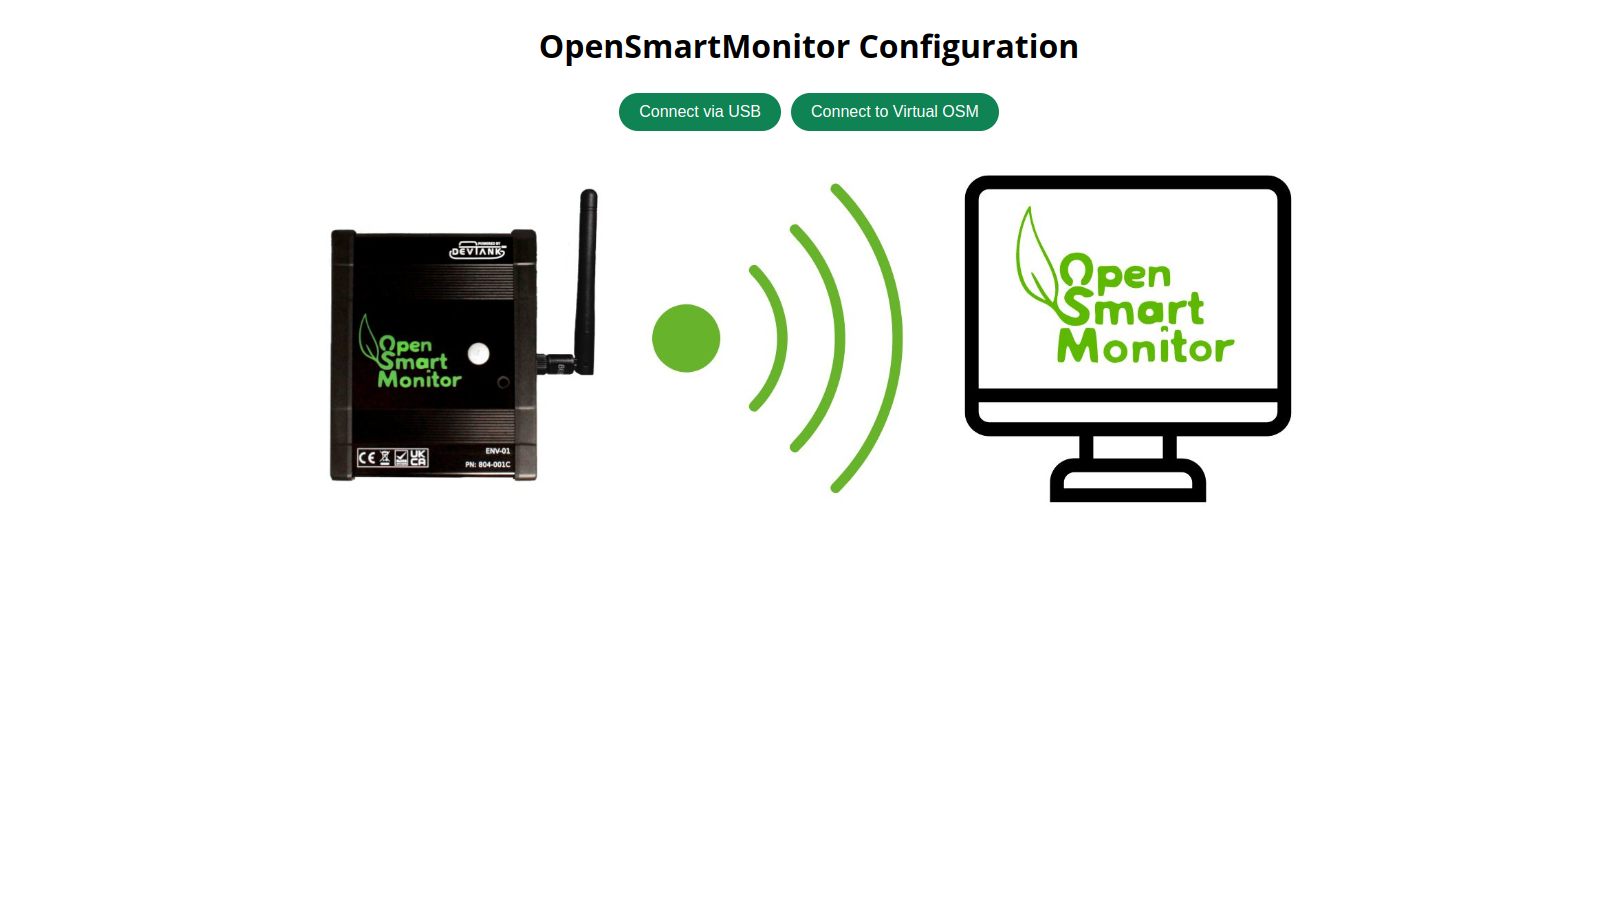
\includegraphics[width=150mm]{Images/connect_page.png}
	\caption{\small Connect page.}
	\label{fig: fig1}
\end{figure}

Connecting will bring you to the home page shown below.

\newpage
\begin{figure}[h]
	\centering
	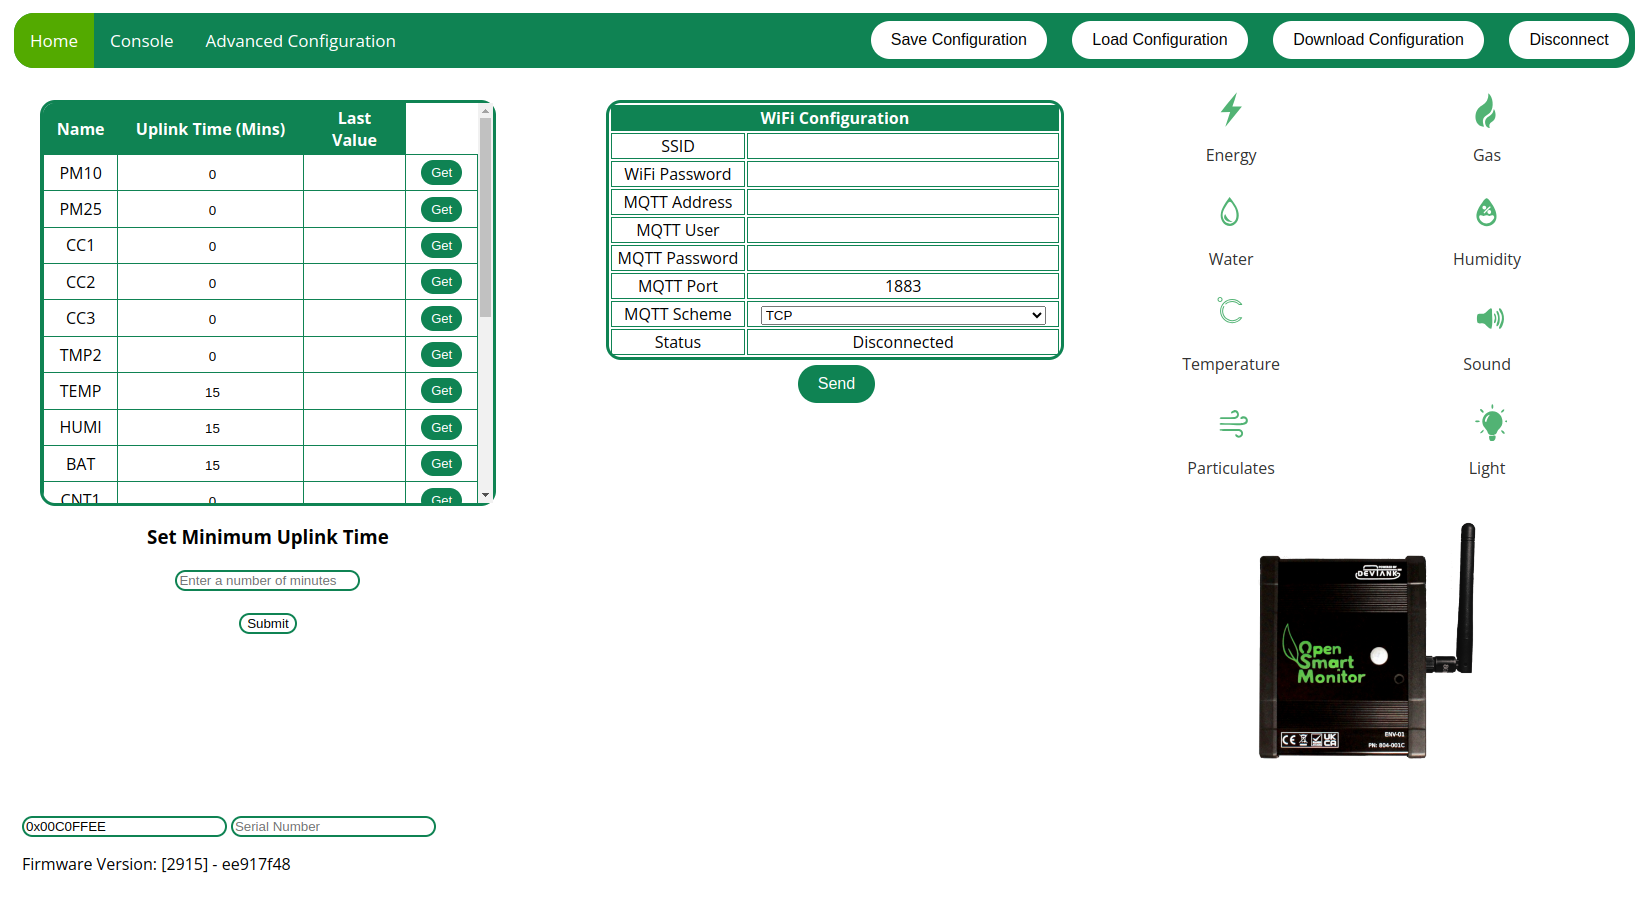
\includegraphics[width=150mm]{Images/home_page.png}
	\caption{\small Home page.}
	\label{fig: fig2}
\end{figure}

\newpage
\section{Wi-Fi Configuration}

\begin{figure}[h]
	\centering
	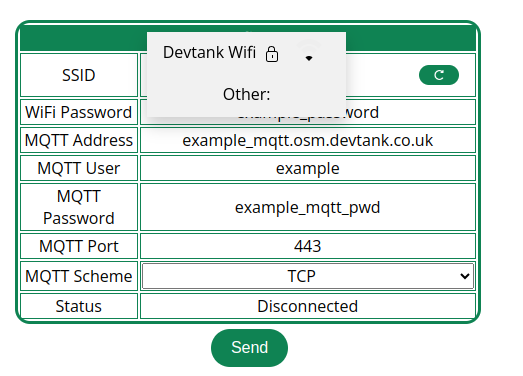
\includegraphics[width=150mm]{Images/wifi_config.png}
	\caption{\small Wi-Fi configuration table.}
	\label{fig: fig3}
\end{figure}

To update the configuration of a Wi-Fi enabled OSM:
\begin{enumerate}
	\item Press the reload symbol in `SSID' to populate the dropdown menu with local networks.
	\item Press `Select Network' to bring up the dropdown menu.
	\item Select the network you want to connect to.
	\item To manually enter a network, select `Other:'.
	\item Edit the rest of the text fields in this table to update the OSM's configuration.
	\item . Press `Send' when you are happy with your changes.
	\item Press `Save Configuration' which is located in the navigation bar.
\end{enumerate}
Bear in mind that spelling mistakes and accidental extra whitespace may cause connection issues, so ensure that you have entered information precisely.

\newpage
\section{LoRaWAN Configuration}

\begin{figure}[h]
	\centering
	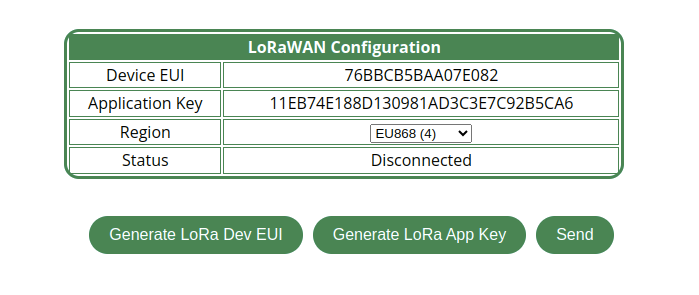
\includegraphics[width=150mm]{Images/lora_config.png}
	\caption{\small LoRaWAN configuration table.}
	\label{fig: fig4}
\end{figure}

To update the configuration of a LoRaWAN enabled OSM:
\begin{enumerate}
	\item Edit the text fields or use the buttons to generate a device EUI and application key.
	\item Press `Send'.
	\item Press `Save Configuration'.
\end{enumerate}

\newpage
\section{Download Configuration}
Downloading the config of your OSM can be useful because if it ever loses it's configuration, you can use this file to write it back. Heavy firmware updates can cause the OSM to lose configuration, so it's recommended to download it before updating the firmware.

This feature also allows you to experiment with the OSM's config as you can use it to restore it to it's original state.

\begin{figure}[h]
	\centering
	
\includegraphics[width=150mm]{Images/download_config.png}
	\caption{\small Navigation bar.}
	\label{fig: fig5}
\end{figure}

To download your OSM's configuration:

\begin{enumerate}
	\item Press `Download Configuration'
	\item Rename the file to something meaningful, such as the OSM's location or serial number.
\end{enumerate}

\newpage
\section{Load Configuration}

\begin{figure}[h]
	\centering
	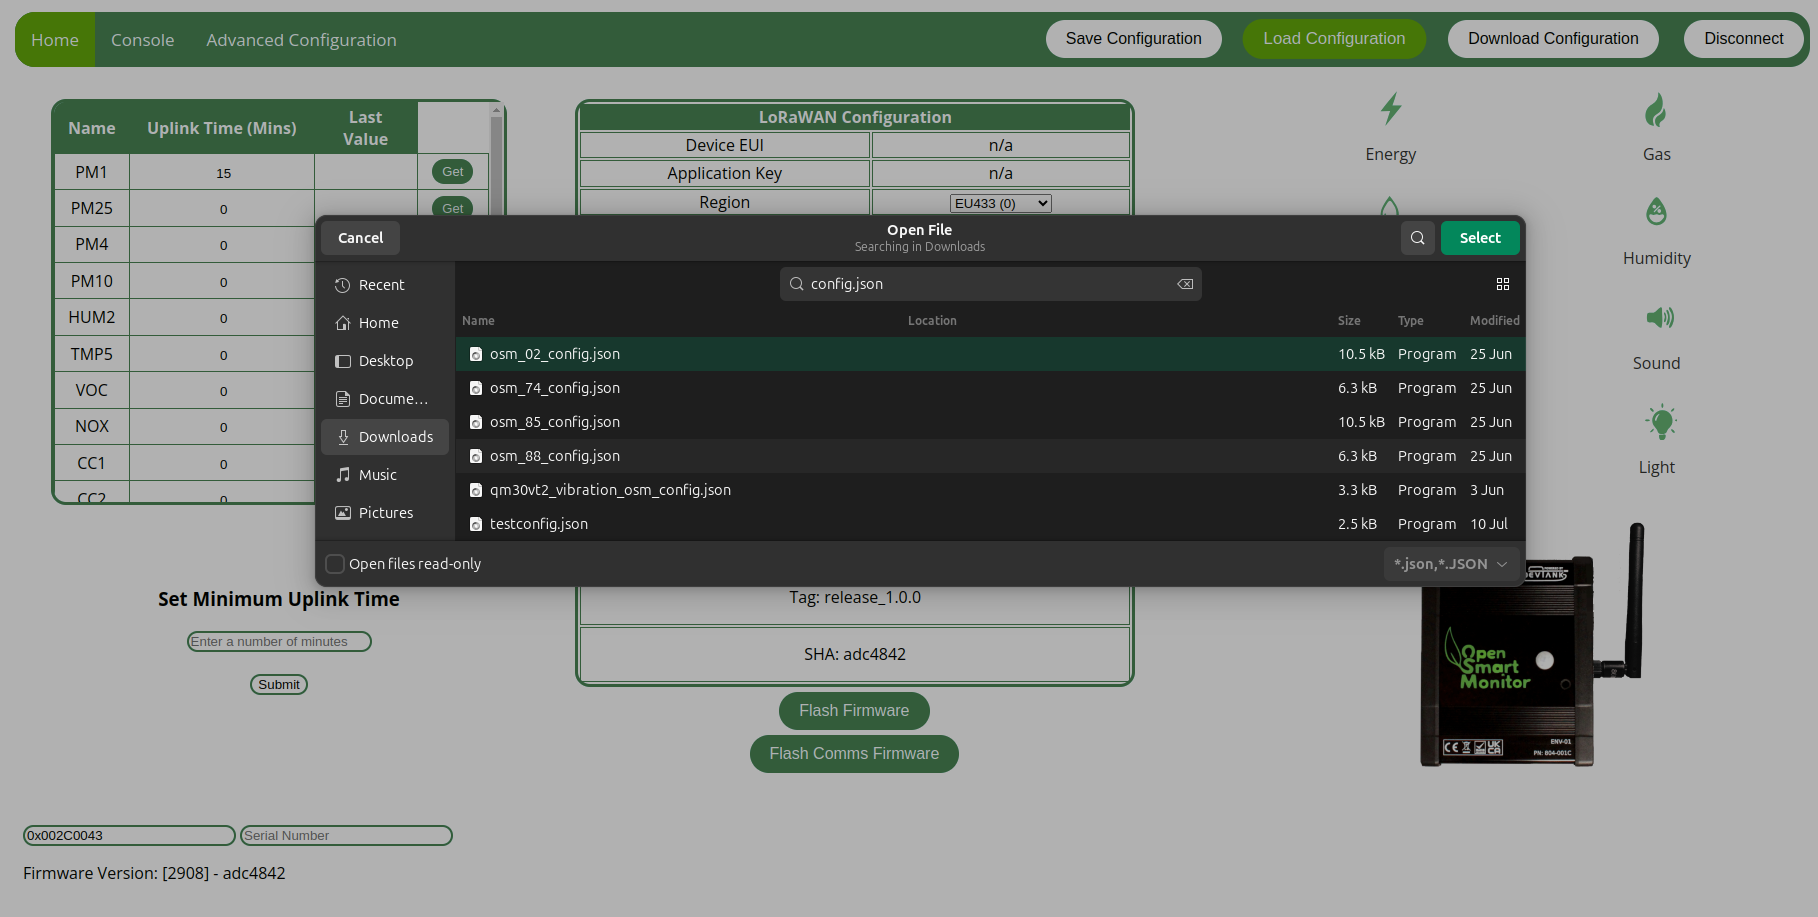
\includegraphics[width=150mm]{Images/load_config.png}
	\caption{\small File selection.}
	\label{fig: fig6}
\end{figure}

To write a configuration file to the OSM:

\begin{enumerate}
	\item Press `Load Configuration'
	\item Select the config file from your file browser.
\end{enumerate}

This will disable the application while it writes the configuration, finally, it will bring you back to the connect page where you will have to reconnect to your OSM.

\newpage
\section{Measurement Configuration}

\begin{figure}[h]
	\centering
	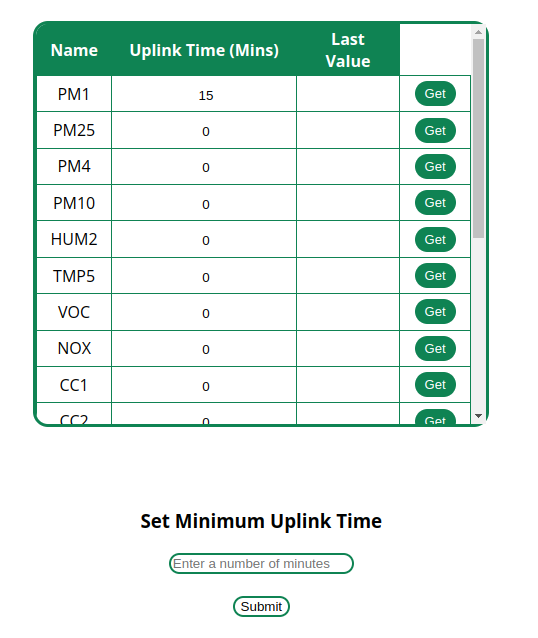
\includegraphics[width=150mm]{Images/measurement_config.png}
	\caption{\small Measurements table.}
	\label{fig: fig7}
\end{figure}

Abbreviations of measurement names are found in the left column. You can hover your mouse over a measurement to get more information.

The number in the `Uplink Time' column represents the amount of minutes/seconds between the OSM sending data for that measurement, the header will tell you the current unit. For example, PM1 is set to 15, therefore every 15 minutes the OSM will send out the collected data.

When a measurement is set to 0, it is essentially turned it off, the OSM will never report its data.

To configure the measurements table:

\begin{itemize}
	\item To update the base minimum uplink time for all measurements, enter a number in the text field under `Set Minimum Uplink Time', then press enter or press `Submit'.
	\item Entering a decimal below 1 such as 0.5 will change the unit to seconds.
	\item To update the uplink time for a singular measurement, edit the text field in the table and enter a number of minutes/seconds.
	\item Remove focus from the text field to send the change.
	\item Press `Save Configuration'.
	\item To read the current value for a measurement, press `Get' in the corresponding row. This will either return a value or `n/a' if it fails to read a measurement, this can occur if the OSM is missing certain hardware. For example, only the OpenSense Air will be able to read temperature, humidity and air quality values.
\end{itemize}

\newpage
\section{Update Firmware}

\begin{figure}[h]
	\centering
	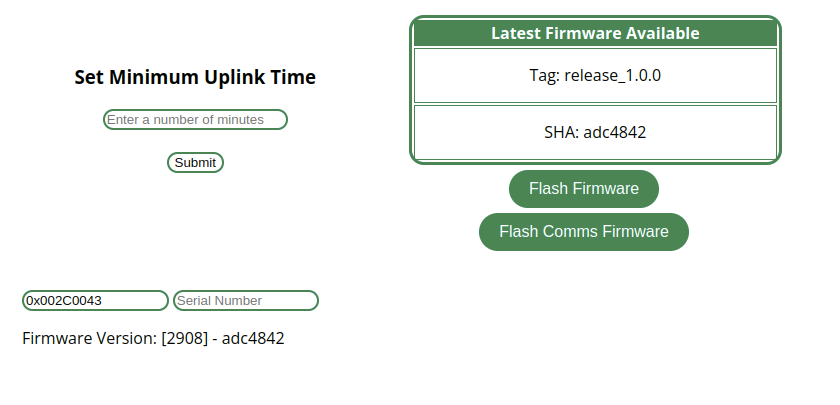
\includegraphics[width=150mm]{Images/flash_firwmare.png}
	\caption{\small Firmware update table.}
	\label{fig: fig8}
\end{figure}

If the SHA in the `Latest Firmware Available' doesn't match the SHA in the `Firmware Version' label in the bottom left of the page, this means you have outdated firmware. The image above shows the firmware versions do match as they are both `adc4842'.

You can update the OSM's firmware by pressing `Flash Firmware'. It's important to download the configuration of your OSM before doing this because you may lose some settings during the firmware update.

Once the firmware update has finished, the page will reload and you will have to reconnect. Check your version now matches the SHA in the table.

\newpage
\section{Update Communication Module Firmware}

To update the firmware for the RAK3172 chip which is responsible for LoRaWAN communications to version 4.1.0, press `Flash Comms Firmware'.

This shouldn't be necessary as your LoRaWAN OSM should already be configured with a v4.1.0 RAK chip.

Flashing the firmware for the ESP module for a Wi-Fi OSM is currently unsupported.

\end{document}